\chapter{Forecasting Short-Term Urban Dynamics: Data Assimilation for Agent-Based Modelling}
\label{ch:malleson_tapper_ward_evans}

\section{Abstract}
\label{malleson:abstract}

\subsection{Background}
\label{malleson:abstract:background}

With such an abundance of real-world data, much research is being undertaken to produce highly accurate models of the current states of urban systems; however, the predictive capabilities of these models is limited.
This general trend also applies to agent-based models (ABMs), owing to the difficulty of incorporating up-to-date data to reduce deviation of model forecasts from reality. 

\subsection{Methods}
\label{malleson:abstract:methods}

The methods contained herein constitute a portion of ongoing work to appropriate data assimilation methods from fields including meteorology, allowing ABMs to incorporate data in real time.
This paper is based on a simple example model of people moving along a street, which is then optimised dynamically using an ensemble Kalman filter in response to hypothetical pedestrian count data.

\subsection{Findings}
\label{malleson:abstract:findings}

\begin{itemize}
    \item data assimilation technique reliably estimates the model parameter that it is attempting to optimise
    \begin{itemize}
        \item how do we measure reliability?
    \end{itemize}
    \item estimates of the `true' system state that are produced by model combined with noisy observations are less accurate than observations in isolation
\end{itemize}

\section{Introduction}
\label{malleson:intro}

With the increasing abundance of high-quality data regarding people's individual activities, there is a growing interest in smart cities --- cities that have the ability to monitor through the use of tech.
However, whilst these smart cities are able to monitor, little has thus far been down to make use of this observation to forecast and react.
It is speculated that this may be as a result of the lack of appropriate methods.

Agent-based models (ABMs) seem to be the most appropriate manner in which to model urban systems; however, calibration of ABMs typically involves the one-off injestion of historical data, then allowing the simulation to progress forward in time, likely diverging from reality and waning in accuracy.

The paper therefore seeks to present a portion of ongoing work that adapts data assimilation techniques such as those found in meteorology to allow ABMs to be optimised by real-time data.
The primary challenge to this approach is that data assimilation techniques are typically designed for systems of differential equations.
The paper presents a simple ABM used to simulate to movement of people moving down a street, which is then dynamically optimised using (hypothetical) pedestrian count data.

\section{Context}
\label{malleson:context}

There is a growing abundance of sensor networks across smart cities.
The aim of this research is to develop methods that suppress error of city-wide models of urban flow in real-time.
This investigation in particular is focussed on the city of Leeds, where policy makers have an interest in encouraging visitors to venture to the south of the city centre; to this end, an ABM has been implemented.
The model represents a pedestrianised throroughfare, where pedestrians are able to enter at one end and leave at the other, with counts of passers-by being taken at each end.
Furthermore, pedestrians are able to leave at some midpoint, without being counted.
The model therefore aims to simulate the movements of the pedestrians, with the count data being used to dynamically suppress error.  

\section{Methods}
\label{malleson:methods}

\subsection{The Agent-Based Model}
\label{malleson:methods:abm}

\begin{itemize}
    \item Using a simple ABM reflecting the scenario portrayed in Section \ref{malleson:context}.
    \item Modelling a one-dimensional street with an entrance point and exit point:
    \begin{itemize}
        \item the entrance is denoted as point A with coordinate 1,
        \item the exit is denoted as point B with coordinate 40,
        \item See figure \ref{fig:malleson_abm_environment}.
    \end{itemize}
    \item The model is Markovian --- Markov definition\ldots
    \item Constant number of agents in model --- 600 for this case.
    \item Agents can be in one of two states:
    \begin{itemize}
        \item Active --- moving from point A to point B with a rate of one coordinate per iteration.
        \item Retired --- present in the model, but not active in the street. In this situtation, the agent has a null position, $N$.
    \end{itemize}
    \item All active agents occupy one of the 40 cells.
    \item Hypothetical footfall cameras located at A and B record entry and exit, giving hourly counts.
    \item State vector contains:
    \begin{itemize}
        \item agent location, $\left( x , y \right)$,
        \item bleed out rate, $r$,
        \item camera count at A,
        \item camera count at B.
    \end{itemize}
    \item Each iteration corresponds to one real minute.
    \item Every hour, a certain number of agents go from N to A (i.e. they become active, having previously been retired).
    \item A midpoint exit exists in the street denoted as M, at $\left( 0, 24 \right)$.
    \begin{itemize}
        \item This allows agents to exit the street without being captured by the camera at B.
        \item Agents reaching M will be returned to N with probability $r$; else they continue their journey.
    \end{itemize}
    \item The rate of entry at A is set for each hour (distributed approximately normal, peak at midday), and does not change day to day.
\end{itemize}

\begin{figure}
  \centering
    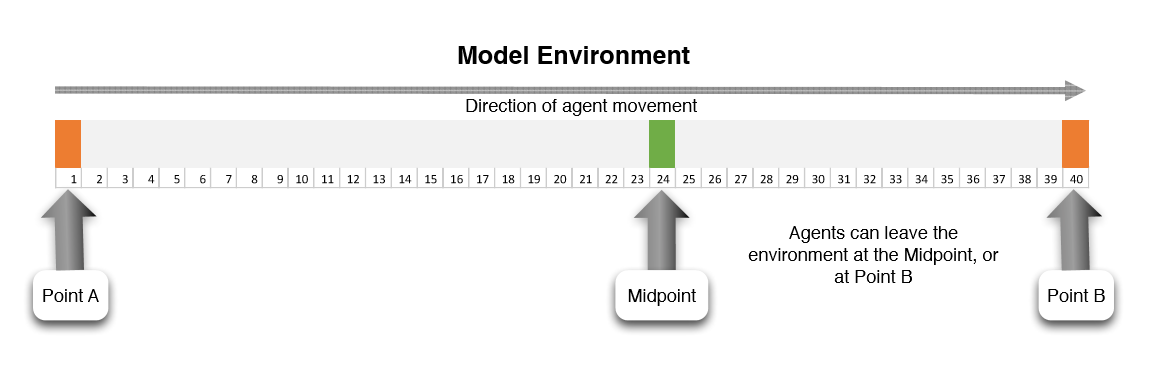
\includegraphics[width=\textwidth]{malleson_abm_environment.png}
  \caption{ABM environment.}
  \label{fig:malleson_abm_environment}
\end{figure}

\subsection{The Ensemble Kalman Filter (EnKF)}
\label{malleson:methods:enkf}

\begin{itemize}
    \item Standard method for data assimilation in meteorology
    \item The method makes use of noisy observations and a model representation of system to produce estimates of the true system state.
    \item Achived by combining the observations with model forecasts, weighting influence by uncertainty --- the adjusted estimate should be more accurate than the observations.
    \item The EnKF maintains an ensemble (thus the name) of estimated model states, which is typically initialised with real-world data.
    \item Each model state then iterates forward in time using the steps:
    \begin{enumerate}
        \item Forecast step,
        \item Data assimilation step,
    \end{enumerate}
    which are outlined as follows in Sections \ref{methods:enkf:forecast} and \ref{methods:enkf:assimilation}.
\end{itemize}

\subsubsection{The forecast step}
\label{methods:enkf:forecast}

\begin{itemize}
    \item Each model in the ensemble is run forward until the next set of observation data becomes available, producing a set of system state forecasts.
    \item The forecasted ensemble mean gives an estimate of the true state.
    \item The forecasted ensemble covariance gives a measure of the uncertainty.
\end{itemize}

\subsubsection{The data assimilation step}
\label{methods:enkf:assimilation}

\begin{itemize}
    \item The ensemble analysis is produced, i.e. the updated ensemble forecasts given the observations.
    \item The ensemble analysis mean gives the best estimate of the true state.
    \item The ensemble analysis covariance gives a measure of the uncertainty.
\end{itemize}

\subsection{Application of the EnKF to the ABM}
\label{malleson:methods:application}

\subsubsection{Hypothetical `Real World' Data}
\label{methods:application:data}

\subsubsection{The Forecast Step}
\label{methods:application:forecast}

\subsubsection{The Data Assimilation Step}
\label{methods:applicaiton:assimilation}

\subsubsection{\ldots and repeat \ldots}
\label{methods:application:repeat}

\section{Results}
\label{malleson:results}

\begin{itemize}
    \item Aim to assess how successful the enKF has been at:
    \begin{itemize}
        \item prediction of footfall at point B,
        \item estimation of bleed out rate, $r$.
    \end{itemize}
    \item Results for virtual observation error of $\mu=0$, $\sigma^2 = 5$:
    \begin{itemize}
        \item analysis is very close to both the truth and virtual observations,
        \item the Kalman filter quickly settles on an accurate estimation of $r$.
    \end{itemize}
    \item Error assessed using the RMSE:
    \begin{itemize}
        \item Forecast: $9.80$
        \item Analysis: $2.58$
        \item Observation: $0.91$
    \end{itemize}
    \item Expected analysis to be smallest as model system converges on real system
    \begin{itemize}
        \item Could be because of the level of randomness in the model
    \end{itemize}
    \item Otherwise, the parameter estimation seems to work ok.
\end{itemize}

\section{Conclusions and Future Outlook}
\label{malleson:conclusion}

\begin{itemize}
    \item Paper presents recent results from ongoing project focussing on the implementation of data assimilation methods for ABMs.
    \item In particular, using an ensemble Kalman Filter for paraemter estimation.
    \item The aim to develop methods to assimilation data streamed in real time.
\end{itemize}